\subsection{A{[}X{]}与一个A-模自同态相伴的模}

设M是一个A-模，u是M的一个自同态。考虑 A 上一个未定元 X 的多项式环 A{[}X{]} 。对于每个多项式 \(p \in A[X]\) 以及所有 \(x \in M\) ，我们记

\[
p. x = p (u) (x).\tag{43}
\]

由于 \((pq)(u) = p(y) \circ q(u)\) （对 A{[}X{]} 中的两个多项式 p、q 成立），这样就在 M 上定义了一个 A{[}X{]}-模结构；集合 M 连同此结构将记作 \(M_{u}\) ；M 上给定的 A-模结构是把 \(M_{u}\) 的算子环限制到 A 而得到的。注意， \(M_{u}\) 的子模正是在 u 下稳定的 M 的子模。

由于映射 \((p, x) \mapsto p \cdot x\) （从 \(\mathbf{A}[\mathbf{X}] \times \mathbf{M}\) 到 \(\mathbf{M}\) ）是 A-双线性的，因此它典范地定义了一个 A-线性映射 \(\phi: \mathbf{A}[\mathbf{X}] \otimes_{\mathbf{A}} \mathbf{M} \to \mathbf{M}\) ，使得

\[
\phi (p \otimes x) = p. x = p (u) (x).\tag{44}
\]

另一方面，A{[}X{]} \(\otimes_{\mathbf{A}}\) M 典范地具有一个 A{[}X{]}-模结构（II，§5，第1号）；我们将把这个 A{[}X{]}-模记作 M{[}X{]}；映射 \(\phi: \mathrm{M}[\mathrm{X}] \to \mathrm{M}_u\) 是 A{[}X{]}-线性的，因为对于 \(p, q\) （在 A{[}X{]} 中）和 \(x \in \mathbf{M}\) ，

\[
\phi (q (p \otimes x)) = \phi ((q p) \otimes x) = (q p). x = q (u) (p (u) (x)) = q. \phi (p \otimes x).
\]

此外， \(u\) 是一个 A{[}X{]}-自同态（ \(\mathbf{M}_u\) 的），因为

\[
u (p. x) = u (p (u) (x)) = (u p (x)) (x) = p. u (x).
\]

最后，一个 A{[}X{]}-自同态 \(\bar{u}\) （M{[}X{]} 的）由写下（II，§ 5，第 1 号）来定义

\[
\bar {u} (p \otimes x) = p \otimes u (x).\tag{45}
\]

此外，由公式 (44) 和 (45) 可推出，诸 A{[}X{]}-线性映射 u, \(\bar{u}\) 和 \(\phi\) 满足关系

\[
\phi \circ \bar {u} = u \circ \phi .\tag{46}
\]

设 \(\psi\) 表示 A{[}X{]}-自同态 \(\mathbf{X} - \bar{\boldsymbol{u}}\) （M{[}X{]} 的），它使得 \(\psi(p \otimes x) = (\mathrm{X}p) \otimes x - p \otimes u(x)\) 。我们有如下命题：

命题 18. A{[}X{]}-同态的序列

\[
\mathbf {M} [ \mathbf {X} ] \stackrel {\psi} {\longrightarrow} \mathbf {M} [ \mathbf {X} ] \stackrel {\phi} {\longrightarrow} \mathbf {M} _ {u} \longrightarrow 0\tag{47}
\]

是正合的。

由于 \(\phi(1 \otimes x) = x\) （对所有 \(x \in \mathbf{M}\) ），显然 \(\phi\) 是满射；另一方面，

\[
\phi (\mathbf {X} (p \otimes x)) = \mathbf {X}. \phi (p \otimes x) = u (\phi (p \otimes x)),
\]

换言之， \(\phi \circ \mathbf{X} = u \circ \phi = \phi \circ \bar{u}\) （由 (46)）；这证明了 \(\phi \circ \psi = 0\) 。还需验证 \(\operatorname{Ker} \phi \subset \operatorname{Im} \psi\) 。为此注意到，由于单项式 \(\mathbf{X}^k\) ( \(k \geqslant 0\) )构成 A-模 \(\mathbf{A}[\mathbf{X}]\) 的一组基，每个元素 \(z \in \mathbf{M}[\mathbf{X}]\) 可以唯一地写成形式 \(z = \sum_k \mathbf{X}^k \otimes x_k\) ，其中 \((x_k)\) 是 \(\mathbf{M}\) 中元素的一个有限支撑族。若 \(z \in \operatorname{Ker} \phi\) ，则 \(\phi(z) = \sum_k u^k(x_k) = 0\) ，且我们可以写成

\[
z = \sum_ {k} \left(\mathrm{X} ^ {k} \otimes x _ {k} - 1 \otimes u ^ {k} (x _ {k})\right) = \sum_ {k} \left(\mathrm{X} ^ {k} - \bar {u} ^ {k}\right) (1 \otimes x _ {k}).
\]

但由于 A{[}X{]}-自同态 X 与 \(\bar{u}\) （M{[}X{]} 的）可交换，则

\(X^{k}-\bar{u}^{k}=(X-\bar{u})\circ\left(\sum_{j=0}^{k-1}X^{j}\bar{u}^{k-j-1}\right)\) 这证明了存在一个 \(y\in M[X]\) ，使得 \(z=\psi(y)\) 。

现在设 \(\mathbf{M}'\) 是另一个 A-模，且 \(u'\) 是 \(\mathbf{M}'\) 的一个自同态；设 \(\mathbf{M}_{u'}^{\prime}\) , \(\phi', \bar{u}', \psi'\) 是由 \(\mathbf{M}'\) 和 \(u'\) 得到的模与映射，就像 \(\mathbf{M}_u\) , \(\phi, \bar{u}, \psi\) 由 \(\mathbf{M}\) 和 \(u\) 得到的那样。那么：

命题 19. 为使映射 \(g\) （ \(\mathbf{M}\) 到 \(\mathbf{M}'\) 的）是 \(\mathrm{A}[\mathrm{X}]\) -同态（ \(\mathbf{M}_u\) 到 \(\mathbf{M}_u'\) 的），必要且充分的是 \(g\) 为 A-同态（ \(\mathbf{M}\) 到 \(\mathbf{M}'\) 的），使得 \(g \circ u = u' \circ g\) 。当如此时，若 \(\bar{g}\) 是 \(\mathrm{A}[\mathrm{X}]\) -同态（ \(\mathbf{M}[\mathrm{X}]\) 到 \(\mathbf{M}'[\mathrm{X}]\) 的、等于 \(1_{\mathbf{A}[X]} \otimes g\) 的）（II，§5，第1号），则图表

\begin{enumerate}
\def\labelenumi{(\arabic{enumi})}
\setcounter{enumi}{47}
\tightlist
\item
\end{enumerate}

\pandocbounded{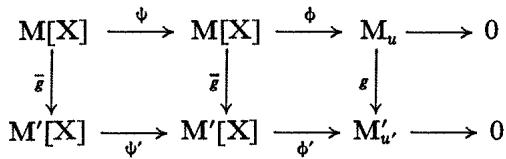
\includegraphics[keepaspectratio]{images/part004_f53e3a23.jpg}}

是交换的。

条件 \(g \circ u = u' \circ g\) 由 (43) 显然是使 \(g\) 成为 A{[}X{]}-同态的必要条件；它是充分的，因为它由归纳法蕴含 \(g \circ u^n = u'^n \circ g\) （对每个整数 \(n > 0\) ）。另一方面，对于所有 \(x \in M\) 以及所有 \(p \in A[X]\) ，

\[
\phi^ {\prime} (\bar {g} (p \otimes x)) = \phi^ {\prime} (p \otimes g (x)) = p (u ^ {\prime}) (g (x)) = g (p (u) (x)) = g (\phi (p \otimes x))
\]

和

\[
\bar {u} ^ {\prime} (\bar {g} (\boldsymbol {p} \otimes x)) = \bar {u} ^ {\prime} (\boldsymbol {p} \otimes g (x)) = \boldsymbol {p} \otimes u ^ {\prime} (g (x)) = \boldsymbol {p} \otimes g (u (x)) = \bar {g} (\bar {u} (\boldsymbol {p} \otimes x))
\]

这证明了图表(48)的交换性。

